%!TEX encoding = UTF-8 Unicode
\documentclass{lecturenotes}

\renewcommand{\vecka}{6}
\newcommand{\veckotema}{Mönster och felhantering}

%!TEX encoding = UTF-8 Unicode
\setbeamertemplate{footline}[frame number]

\newcommand{\LibVersion}{0.1.0} % latest version of introlib at https://github.com/lunduniversity/introprog-scalalib
\newcommand{\LibJar}{\texttt{introprog-\LibVersion.jar}}
\newcommand{\JDKApiUrl}{\url{https://docs.oracle.com/javase/8/docs/api/}}


\title[Föreläsningsanteckningar EDAA45, \CurrentYear]{EDAA45 Programmering, grundkurs}
\subtitle{Läsvecka \vecka: \veckotema}
\author{Björn Regnell}
\institute{Datavetenskap, LTH}
\date{Lp1-2, HT \CurrentYear}

%!TEX encoding = UTF-8 Unicode

\newcommand{\ModWeekONE}{Introduktion}
\newcommand{\ExeWeekONE}{expressions}
\newcommand{\LabWeekONE}{kojo}


\newcommand{\ModWeekTWO}{Program, kontrollstrukturer}
\newcommand{\ExeWeekTWO}{programs}
\newcommand{\LabWeekTWO}{--}


\newcommand{\ModWeekTHREE}{Funktioner, abstraktion}
\newcommand{\ExeWeekTHREE}{functions}
\newcommand{\LabWeekTHREE}{irritext}


\newcommand{\ModWeekFOUR}{Objekt, inkapsling}
\newcommand{\ExeWeekFOUR}{objects}
\newcommand{\LabWeekFOUR}{blockmole}


\newcommand{\ModWeekFIVE}{Klasser, datamodellering}
\newcommand{\ExeWeekFIVE}{classes}
\newcommand{\LabWeekFIVE}{--}


\newcommand{\ModWeekSIX}{Mönster, felhantering}
\newcommand{\ExeWeekSIX}{patterns}
\newcommand{\LabWeekSIX}{blockbattle}


\newcommand{\ModWeekSEVEN}{Sekvenser, enumerationer}
\newcommand{\ExeWeekSEVEN}{sequences}
\newcommand{\LabWeekSEVEN}{shuffle}


\newcommand{\ModWeekEIGHT}{Matriser, typparametrar}
\newcommand{\ExeWeekEIGHT}{matrices}
\newcommand{\LabWeekEIGHT}{life}


\newcommand{\ModWeekNINE}{Mängder, tabeller}
\newcommand{\ExeWeekNINE}{lookup}
\newcommand{\LabWeekNINE}{words}


\newcommand{\ModWeekTEN}{Arv, komposition}
\newcommand{\ExeWeekTEN}{inheritance}
\newcommand{\LabWeekTEN}{snake0}


\newcommand{\ModWeekELEVEN}{Kontextuella abstraktioner, api}
\newcommand{\ExeWeekELEVEN}{context}
\newcommand{\LabWeekELEVEN}{snake1}


\newcommand{\ModWeekTWELVE}{Valfri fördjupning, Projekt}
\newcommand{\ExeWeekTWELVE}{extra}
\newcommand{\LabWeekTWELVE}{Projekt0}


\newcommand{\ModWeekTHIRTEEN}{Repetition}
\newcommand{\ExeWeekTHIRTEEN}{examprep}
\newcommand{\LabWeekTHIRTEEN}{Projekt1}


\newcommand{\ModWeekFOURTEEN}{Muntligt prov}
\newcommand{\ExeWeekFOURTEEN}{Munta}
\newcommand{\LabWeekFOURTEEN}{Munta}



\begin{document}

\frame{\titlepage}
\setnextsection{\vecka}
\section[Vecka \vecka: \veckotema]{\veckotema}
\frame{\tableofcontents}

%!TEX encoding = UTF-8 Unicode
%!TEX root = ../lect-w06.tex

%%%

\Subsection{Matchning}

\ifkompendium
\noindent  I ett match-uttryck kan man matcha på ett visst värde eller på en viss typ och match-uttryck används gärna istället för nästlade if-uttryck, då de ofta är lättare att läsa och begripa. Med match-uttryck kan man också göra \Emph{mönstermatchning} mot case-klass-instanser, t.ex. för att på ett smidigt sätt undersöka om attribut har speciella värden. Match-uttryck i Scala är en mer kraftfull variant av \code{switch}-satser som finns i många andra språk.  
\fi

\begin{Slide}{Vad är matchning?}

  \begin{itemize}
    \item Matchning gör man då man vill jämföra ett värde mot andra värden och hitta överensstämmelse \Eng{match} enligt olika \Emph{mönster}.
    \item Med mönster kan man även \Alert{plocka isär} objekt i sina beståndsdelar.
  \end{itemize}
\end{Slide}

\begin{Slide}{Plocka isär ett objekt i sina beståndsdelar med mönster}

\begin{REPLnonum}
scala> case class Point(x: Int, y: Int)

scala> val p = Point(1, 2)      // konstruera en punkt
val p: Point = Point(1,2)
\end{REPLnonum}

\pause 

~\\
\begin{REPLnonum}
scala> val Point(x, y) = p      // plocka isär en punkt
val x: Int = 1
val y: Int = 2
  
\end{REPLnonum}
\end{Slide}


\begin{Slide}{Kolla om det passar med nästlade if-then-else-uttryck}
Ett vanligt problem: \\ att kolla vilket bland många värden som passar \\~\\

Kan göras med nästlade if-then-else-uttryck:

\begin{Code}
val g = scala.io.StdIn.readLine("grönsak:")
val smak =
  if (g == "gurka") "gott!"
  else if (g == "tomat") "jättegott!"
  else if (g == "broccoli") "ganska gott..."
  else "inte gott :("

println(g + " är " + smak)
\end{Code}
      
\end{Slide}


\ifkompendium\else
\begin{SlideExtra}{Matchning är ungefär som att passa klossar i en låda}

\includegraphics[width=0.8\textwidth]{../img/plocklada.png}
\end{SlideExtra}
\fi


\begin{Slide}{Kolla om det passar med \texttt{match}-uttryck}\SlideFontSmall
I stället för nästlade \code{if} kan du använda Scalas kraftfulla \code{match}-\Emph{uttryck}:

\begin{Code}
def g = scala.io.StdIn.readLine("Ange en grönsak: ")
def smak = g match 
  case "gurka"    => "gott!"
  case "tomat"    => "jättegott!"
  case "broccoli" => "ganska gott..."
  case _ => "mindre gott..."
\end{Code}
\begin{itemize}
\pause\item Varje \code{case}-gren testas var för sig i tur och ordning uppifrån och ned.
\item Det som står mellan \code{case} och \code{=>} kallas ett \Emph{mönster} \Eng{pattern}
\item Sista default-grenen ovan kallas \Emph{wildcard-mönster}: \code{case _ => }
\item Ovan är exempel på matchning mot \Emph{konstant-mönster}, \\ i detta fallet tre stycken strängkonstantmönster.
\item Det finns många andra sätt att skriva mönster.
\end{itemize}
% \pause Scalas \code{match} ''faller inte igenom'' som \code{switch}-satser som finns i många språk, t.ex. Java...

\end{Slide}


\begin{Slide}{Matchning med gard}
Man kan stoppa in en s.k \Emph{gard} \Eng{guard} innan pilen \code{=>} för att villkora matchningen: (notera \code{if} utan \code{then})
\begin{Code}
def g = scala.io.StdIn.readLine("Ange en grönsak: ")
def smak = g match 
  case "gurka" if math.random() > 0.5 => "gott ibland!"
  case "tomat" => "jättegott!"
  case "broccoli" => "ganska gott..."
  case _ => "mindre gott..."
\end{Code}
\code{case}-grenen med gard ger bara en lyckad matchning \\ om uttrycket efter \code{if} är sant; annars provas nästa gren, etc.
\end{Slide}

\begin{Slide}{Matchning med variabelmönster}\SlideFontSmall
Om det finns ett namn efter \code{case} som börjar med liten begynnelsebokstav, blir detta namn en variabel som automatiskt binds till uttrycket före \code{match}:

\begin{Code}
def g = scala.io.StdIn.readLine("Ange en grönsak: ")
def smak = g match 
  case "gurka" if math.random() > 0.5 => "gott ibland!"
  case "tomat" => "jättegott!"
  case "broccoli" => "ganska gott..."
  case other => "smakar bakvänt: " + other.reverse
\end{Code}

Ett enkelt variabelmönster, så som \\ \code{case other => ...} \\ i exemplet ovan, matchar \Emph{allt}! \\\code{other} får alltså värdet av \code{g} om \code{g} \Alert{inte} är \code{"gurka"}, \code{"tomat"}, \code{"broccoli"}.

\end{Slide}


\begin{Slide}{Matchning med eller-mönster}\SlideFontSmall
Om man har samma utfall för olika grenar kan dessa slås ihop och mönstret separeras med vertikalstreck: \code{|}
\begin{Code}
def g = scala.io.StdIn.readLine("Ange en grönsak: ")
def smak = g match 
  case "gurka" => "gott"
  case "tomat" => "gott"
  case "lök"   => "gott"
  case _ => "inte gott"
\end{Code}

Mer koncist med eller-mönster:

\begin{Code}
def g = scala.io.StdIn.readLine("grönsak:")
def smak = g match 
  case "gurka" | "tomat" | "lök" => "gott"
  case _ => "inte gott"
\end{Code}



\end{Slide}





\begin{Slide}{Matchning med typade mönster}\SlideFontSmall
Med en typannotering efter en variabel får man ett \Emph{typat mönster} \Eng{typed pattern}. Om matchningen lyckas blir värdet \Alert{omvandlat} till den specifika typen och binds till variabeln.
\begin{Code}
def f = 
  if (math.random() < 0.5) 42 + math.random() else "gurka" + math.random()

def g = f match 
  case x: Double => x.round.toInt
  case s: String => s.length
\end{Code}
\code{f} får typen \code{Matchable} som är subtyp till \code{Any}. Vilken typ får \code{g}? \pause ~~\code{Int}\\
Matchning mot specifika typer enl. ovan används i idiomatisk Scala hellre än \code{isInstanceOf} men man kan göra motsvarande ovan med detta if-uttryck:
\begin{Code}
def g2 =  
  val x = f
  val y = 
    if (x.isInstanceOf[Double]) x.asInstanceOf[Double].round.toInt
    else if (x.isInstanceOf[String]) x.asInstanceOf[String].length
  y.asInstanceOf[Int] // kan detta ge körtidsfel? kan kompilatorn kolla det?
\end{Code}
\end{Slide}

\begin{Slide}{Typen \text{Matchable}}
När ett uttryck inte kan ges en mer specifik typ så härleds \code{Matchable}, vilket visar att värdet kan undersökas med \code{match}.\footnote{Mer detaljer om varför \code{Matchable} behövs här: https://dotty.epfl.ch/docs/reference/other-new-features/matchable.html}
\begin{REPLnonum}
scala> def f = if math.random() > 0.5 then 42 else "hej"
def f: Matchable
\end{REPLnonum}
%Eftersom typen \code{String} och typen \code{Double} inte har något annat gemensamt bli den mest specifika typen som kan härledas \code{Matchable}, som är nästan lika generell som topptypen \code{Any}.
\end{Slide}

\begin{Slide}{Konstruktormönster med case-klasser}\SlideFontSmall
En basklass med gemensamma delar och två subtyper:
\begin{Code}
trait Grönsak:
  def vikt: Int
  def ärRutten: Boolean

case class Gurka(vikt: Int, ärRutten: Boolean) extends Grönsak
case class Tomat(vikt: Int, ärRutten: Boolean) extends Grönsak
\end{Code}
\pause
Tack vare case-klasserna kan man använda \Emph{konstruktormönster} \Eng{constructor pattern} för att se vad som finns \Alert{inuti} en instans:
\begin{Code}
def testa(g: Grönsak): String = g match 
  case Gurka(v, false) => "gott, väger " + v
  case Gurka(_, true)  => "inte gott"
  case Tomat(v, r)     => (if r then "inte " else "") + s"gott, väger $v"
  case _ => "okänd grönsak: $g"
\end{Code}

Konstruktormönster ''\Emph{plockar isär}'' det som matchas och binder variabler till de attribut som finns i case-klassens konstruktor.
\end{Slide}


\begin{Slide}{Plocka isär samlingar med djupa mönster}
Man kan plocka isär innehållet i en samling så här:
\begin{Code}
def visa(xs: Vector[Grönsak]): String = xs match
  case Vector()               => "tom grönsaksvektor"
  case Vector(Gurka(v, true)) => s"en rutten gurka som väger $v"
  case Vector(g)              => s"exakt en grönsak: $g"
  case Vector(g1, g2)         => s"exakt två grönsaker: $g1, $g2"
  case g +: gs                => s"först en $g och sedan svansen: $gs"
\end{Code}
Vad händer om du byter ordning på andra och tredje mönstret?
\end{Slide}

\begin{Slide}{Matchning på tupler}
Det går fint att plocka isär tupler med mönstermatchning:\footnote{\url{https://youtu.be/aboZctrHfK8}}
\begin{Code}
var pair = ("hej", 42)

pair match
  case (a, b) if b == 42 => s"livets mening är funnen: $a"
  case (_, b)            => s"fattas mening: $b"

\end{Code}

\end{Slide}

\begin{Slide}{Mönstermatchning och uppräkning med case-objekt}\SlideFontSmall
En bastyp och specifika singelobjekt av gemensam typ:
\begin{Code}
trait Färg
case object Spader  extends Färg // funkar utan case men vi vill ha najs toString
case object Hjärter extends Färg
case object Ruter   extends Färg
case object Klöver  extends Färg

def parallellFärg(f: Färg): Färg = f match
  case Spader  => Klöver
  case Klöver  => Spader
  case Hjärter => Ruter
\end{Code}
Vilken case-gren har vi glömt? Kan kompilatorn hjälpa oss?
\pause
\begin{REPL}
scala> parallellFärg(Ruter)
scala.MatchError: Ruter 
\end{REPL}
\Alert{Undantag vid körtid} \code{:(}
\end{Slide}

\begin{Slide}{Mönstermatchning och förseglade typer}\SlideFontSmall
Med nyckelordet \code{sealed} får vi en kompileringsvarning.
\begin{Code}
sealed trait Färg //tryck Alt+Enter i REPL för tolkning av flera rader ett svep
case object Spader  extends Färg
case object Hjärter extends Färg
case object Ruter   extends Färg
case object Klöver  extends Färg

def parallellFärg(f: Färg): Färg = f match 
  case Spader  => Klöver
  case Klöver  => Spader
  case Hjärter => Ruter
\end{Code}
\begin{REPL}
1 |def parallellFärg(f: Färg): Färg = f match 
  |                                   ^
  |                           match may not be exhaustive.
  |
  |                           It would fail on pattern case: Ruter
def parallellFärg(f: Färg): Färg
\end{REPL}
\Emph{Varning vid kompilering} \code{:)} ~~~Sista raden visar att det bara är en varning!
\end{Slide}

\begin{Slide}{Mönstermatcha enumeration}\SlideFontSmall
I stället för \code{sealed trait ... case object ...} kan du använda en \Emph{enumeration} (ä.k. uppräkning, uppräknad datatyp, \Eng{enumeration}).
\begin{Code}
enum Färg:
  case Spader, Hjärter, Ruter, Klöver
  
def parallellFärg(f: Färg): Färg = 
  import Färg.*
  f match 
    case Spader  => Klöver
    case Klöver  => Spader
    case Hjärter => Ruter
\end{Code}
\pause
\begin{REPL}
def parallellFärg(f: Färg): Färg
3 |  f match 
  |  ^
  |  match may not be exhaustive.
  |
  |  It would fail on pattern case: Ruter
\end{REPL}
\Emph{Även här får vi hjälpsam varning vid kompilering} \code{:)} 
\end{Slide}

\begin{Slide}{Stora/små begynnelsebokstäver vid matchning}
\Alert{Fallgrop}: matcha \Alert{värde} som börjar med \Alert{liten} bokstav.
\begin{REPL}
scala> val livetsMening = 42

scala> def ärLivetsMeningBuggig(svar: Int) = svar match 
         case livetsMening => true    // lokalt namn som matchar allt!
         case _ => false

scala> ärLivetsMeningBuggig(43)
val res0: Boolean = true

scala> val LivetsMening = 42   // stor begynnelsebokstav

scala> def ärLivetsMening(svar: Int) = svar match 
         case LivetsMening => true    // funkar fint!
         case _ => false

scala> ärLivetsMening(43)
val res1: Boolean = false
\end{REPL}
\end{Slide}


\begin{Slide}{Stora/små begynnelsebokstäver vid matchning}
Ett sätt att komma runt problemet med liten begynnelsebokstav: \\
\Emph{backticks} to the rescue!
\begin{REPL}
scala> val livetsMening = 42

scala> def ärLivetsMeningBackTicks(svar: Int) = svar match 
         case `livetsMening` => true    // nu funkar det!
         case _ => false

scala> ärLivetsMeningBackTicks(43)
val res2: Boolean = false
\end{REPL}
\end{Slide}


\begin{Slide}{Mönster på andra ställen än i \texttt{match}}\SlideFontSmall
Mönster i \Emph{deklarationer}:
\vspace{-0.25em}\begin{REPL}
scala> case class Point(x: Int, y: Int)

scala> val p = Point(0, 1)

scala> val Point(x, y) = p          // konstruktormönster med case-klass
val x: ???
val y: ???

scala> val (x, y, z) = (0, 1, 2)    // konstruktormönster med tupel
val x: ???
val y: ???
val z: ???

\end{REPL}
Mönster i \Emph{for-satser}:
\vspace{-0.25em}\begin{REPL}
scala> val xs = for (x, y) <- Vector((1,2), (3,4)) yield x
val xs: ???
\end{REPL}

\end{Slide}

\begin{Slide}{Mönster på andra ställen än i \texttt{match}}\SlideFontSmall
Mönster i \Emph{deklarationer}:
\vspace{-0.25em}\begin{REPL}
scala> case class Point(x: Int, y: Int)

scala> val p = Point(0, 1)

scala> val Point(x, y) = p          // konstruktormönster med case-klass
val x: Int = 0
val y: Int = 1

scala> val (x, y, z) = (0, 1, 2)    // konstruktormönster med tupel
val x: Int = 0
val y: Int = 1
val z: Int = 2

\end{REPL}
Mönster i \Emph{for-satser}:
\vspace{-0.25em}\begin{REPL}
scala> val xs = for (x, y) <- Vector((1,2), (3,4)) yield x
val xs: Vector[Int] = Vector(1, 3)
\end{REPL}
\end{Slide}

\begin{Slide}{Fördjupning om mönster}\SlideFontSmall
\begin{itemize}
\item binda variabler till mönsterdelar med \code{@} \\
\code{case Vector(xs@Vector(a), Vector(42)) => ...}

\item sekvensmönster med \code{_}, \code{xs*} och \code{_*} 
\\ \code{case Vector(a, _, c) => ... }  matchar om 3 element, \_ kvittar
\\ \code{case Vector(a, svans*) => ... }  matchar om minst ett element
\\ \code{case Vector(a, _*) => ... }  intresserad av första, svans kvittar

\item Partiella funktioner med \code{case} utan \code{match}: \code|val pf: Int => Double = { case z if z != 0 => 1/z }| \\ Notera att klammerparenteserna behövs för att skapa partiell funktion med \code{case} utan \code{match}. Funktionen är inte definierad för argumentet \code{0}:

\begin{REPLsmall}
scala> pf(0)                         
scala.MatchError: 0 
\end{REPLsmall}
Detta är användbart vid iterering över samling med \code{collect}: \\\code|xs.collect{ case (a,b) if a > 0 => a }|  
\item Läs mer om mönster här: \\\url{https://docs.scala-lang.org/scala3/book/control-structures.html}

% \item Läs mer om mönster här:  \href{http://www.artima.com/pins1ed/case-classes-and-pattern-matching.html}{\SlideFontTiny www.artima.com/pins1ed/case-classes-and-pattern-matching.html}

% \item För djupare förståelse av hur \code{case} fungerar, läs speciellt om \Emph{partiella funktioner} här: \href{http://www.artima.com/pins1ed/case-classes-and-pattern-matching.html\#15.7}{\SlideFontTiny www.artima.com/pins1ed/case-classes-and-pattern-matching.html\#15.7}

% \item Läs om extractors här: \href{http://www.artima.com/pins1ed/extractors.html}{\SlideFontTiny www.artima.com/pins1ed/extractors.html}

\end{itemize}
\end{Slide}


\begin{Slide}{Fördjupning: metoden \texttt{unapply}}\SlideFontSmall
När du deklarerar en case-klass kommer kompilatorn att \Alert{automatiskt generera en metod} med namnet \Emph{\texttt{unapply}}.
\begin{REPL}
scala> case class Gurka(vikt: Int, ärRutten: Boolean)

scala> Gurka.unapply // tryck ENTER för att se typen
val res0: Gurka => Gurka = Lambda1914/0x00000008408cf840@b0e7bde

scala> val g = Gurka(100, false)

scala> Gurka.unapply(g)
val res1: Gurka = Gurka(100,false)
\end{REPL}
Vad ska detta vara bra för? \\\pause
\code{unapply} genereras av kompilatorn och används internt vid matchning och det är den metoden som gör att case-klasser kan användas i konstruktormönster. \\Principen är generell: Man kan skapa \Emph{egna} s.k. \Alert{extraktorer} \Eng{extractors} som kan plocka isär ett värde med mönstermatchning, genom att definiera en egen \code{unapply}.
\end{Slide}

%!TEX encoding = UTF-8 Unicode
%!TEX root = ../lect-w06.tex

%%%


\ifkompendium\else
%\Subsection{Kapsla in speciella värden: Option[kanske saknas] och Try[kanske misslyckas]}
\Subsection{Hantera speciella värden med inkapsling}

{
\setbeamertemplate{navigation symbols}{}
\setbeamercolor{background canvas}{bg=black}
\begin{frame}[plain]
    \color{white}{Inkapsling av speciella värden så att krasch kan undvikas}
    \makebox[\linewidth]{
\includegraphics[width=\paperwidth]{../img/crystal.jpg}}
\end{frame}
}
\fi

\Subsection{Hantera saknade värden med \texttt{Option}}

\begin{Slide}{Hur hantera saknade värden?}\SlideFontSmall
Olika sätt att hantera saknade värden:
\begin{itemize}
\item Hitta på ett specialvärde: exempel -1 för saknat värde
\item \code{null} om värde saknas (vanligt i Java m.fl. språk, mkt ovanligt i Scala)
\item Använd en samling och låt tom samling representera saknat värde: \\
\code{val sums = Vector(Vector(42),Vector(32),Vector(),Vector(21))}

\item \code{Option[A]} gemensam bastyp för: \\
  \code{None} som representerar \Alert{saknat värde}, och \\ \code{Some[A]} som representerar att \Emph{värde finns}
\end{itemize}
\end{Slide}



\begin{Slide}{En gemensam bastyp för ett värde som kanske saknas}\SlideFontSmall\ifkompendium\footnotesize\fi
\vspace{-0.0em}\begin{center}
\newcommand{\TextBox}[1]{\raisebox{0pt}[1em][0.5em]{#1}}
\tikzstyle{umlclass}=[rectangle, draw=black,  thick, anchor=north, text width=3cm, rectangle split, rectangle split parts = 3]
\begin{tikzpicture}[inner sep=0.5em]
\node [umlclass, rectangle split parts = 2, xshift=0cm, text width=3.5cm] (BaseType)  {
            \textit{\textbf{\centerline{\TextBox{\code{Option[A]}}}}}
            \nodepart[]{second}
            \TextBox{\code{def get: A}}\newline
            \TextBox{\code{def isEmpty: Boolean}}

        };

\node [umlclass, rectangle split parts = 1]  at (-2.5cm,-3.0cm) (SubType1) {
            \textbf{\centerline{\TextBox{\code{Some[A]}}}}
            % \nodepart[]{second} \TextBox{\code{val x: A}}
        };

\node [umlclass, rectangle split parts = 1] at (2.5cm,-3.0cm) (SubType2)  {
            \textbf{\centerline{\TextBox{\code{None}}}}
        };
\draw[umlarrow] (SubType1.north) -- ++(0,0.5) -| (BaseType.south);
\draw[umlarrow] (SubType2.north) -- ++(0,0.5) -| (BaseType.south);
\end{tikzpicture}
\end{center}
\pause
\vspace{-0.5em}\begin{REPL}
scala> var x: Option[Int] = Some(42)

scala> x.isEmpty
val res0: Boolean = false

scala> x = None

scala> x.isEmpty
val res1: Boolean = true
\end{REPL}
\end{Slide}


\begin{Slide}{Option för hantering av ev. saknade värden}\SlideFontSmall
Alla vill inte berätta för Facebook vad de har för kön. \\ Förbättra Facebooks kod med ett litet Scala-program:
\begin{Code}
enum Gender:
  case Male, Female

case class Person(name: String, gender: Option[Gender])
\end{Code}
\pause
\begin{REPL}
scala> val p1 = Person("Björn",  Some(Gender.Male))
scala> val p2 = Person("Sandra", Some(Gender.Female))
scala> val p3 = Person("Kim",  None)
scala> val g2 = p2.gender
scala> def show(g: Option[Gender]): String = g match {
         case Some(x) => x.toString
         case None    => "unknown"
       }
scala> show(g2)
scala> show(p3.gender)
scala> val ps = Vector(p1,p2,p3)
scala> ps.map(_.gender).map(show)   // None ignoreras av map
\end{REPL}
\end{Slide}

\begin{Slide}{Några smidiga metoder på \code{Option}}\SlideFontSmall
Metoden \code{getOrElse} gör att man ofta kan undvika matchning.
\begin{Code}
var opt: Option[Int] = None

val x = opt.getOrElse(42)      // get the value or give a default if missing
\end{Code}

Flera av de vanliga samlingsmetoderna funkar, t.ex. \code{foreach} och \code{map}.
\begin{Code}
opt.foreach{x => println(x)}    // only done if value exists

opt.map{x => x + 1}             // only done if value exists

opt = Some(42)                  // change opt to now have some value

opt.foreach{x => println(x)}    // done as value now exists

opt.map{x => x + 1}             // done as value now exists

\end{Code}
\end{Slide}


\begin{Slide}{Några samlingsmetoder som ger en \code{Option}, övning}
\begin{REPL}
scala> val (xs, ys) = (Vector(1,2,3), Vector())

scala> xs.headOption
res0: ???

scala> ys.headOption
res1: ???

scala> xs.find(_ > 1)
res2: ???

scala> xs.find(_ > 5)
res3: ???

scala> val huvudstad = Map("Sverige" -> "Sthlm", "Skåne" -> "Malmö")

scala> huvudstad.get("Skåne")
res4: ???

scala> huvudstad.get("Danmark")
res5: ???
\end{REPL}
\end{Slide}

\begin{Slide}{Några samlingsmetoder som ger en \code{Option}, svar}
\begin{REPL}
scala> val (xs, ys) = (Vector(1,2,3), Vector())

scala> xs.headOption
res0: Option[Int] = Some(1)

scala> ys.headOption
res1: Option[Nothing] = None

scala> xs.find(_ > 1)
res2: Option[Int] = Some(2)

scala> xs.find(_ > 5)
res3: Option[Int] = None

scala> val huvudstad = Map("Sverige" -> "Sthlm", "Skåne" -> "Malmö")

scala> huvudstad.get("Skåne")
res4: Option[String] = Some(Malmö)

scala> huvudstad.get("Danmark")
res5: Option[String] = None
\end{REPL}
\end{Slide}

%!TEX encoding = UTF-8 Unicode
%!TEX root = ../lect-w06.tex

%%%



\Subsection{Undantag}

\ifkompendium\else
\begin{SlideExtra}{Undantag kan orsaka krasch...}
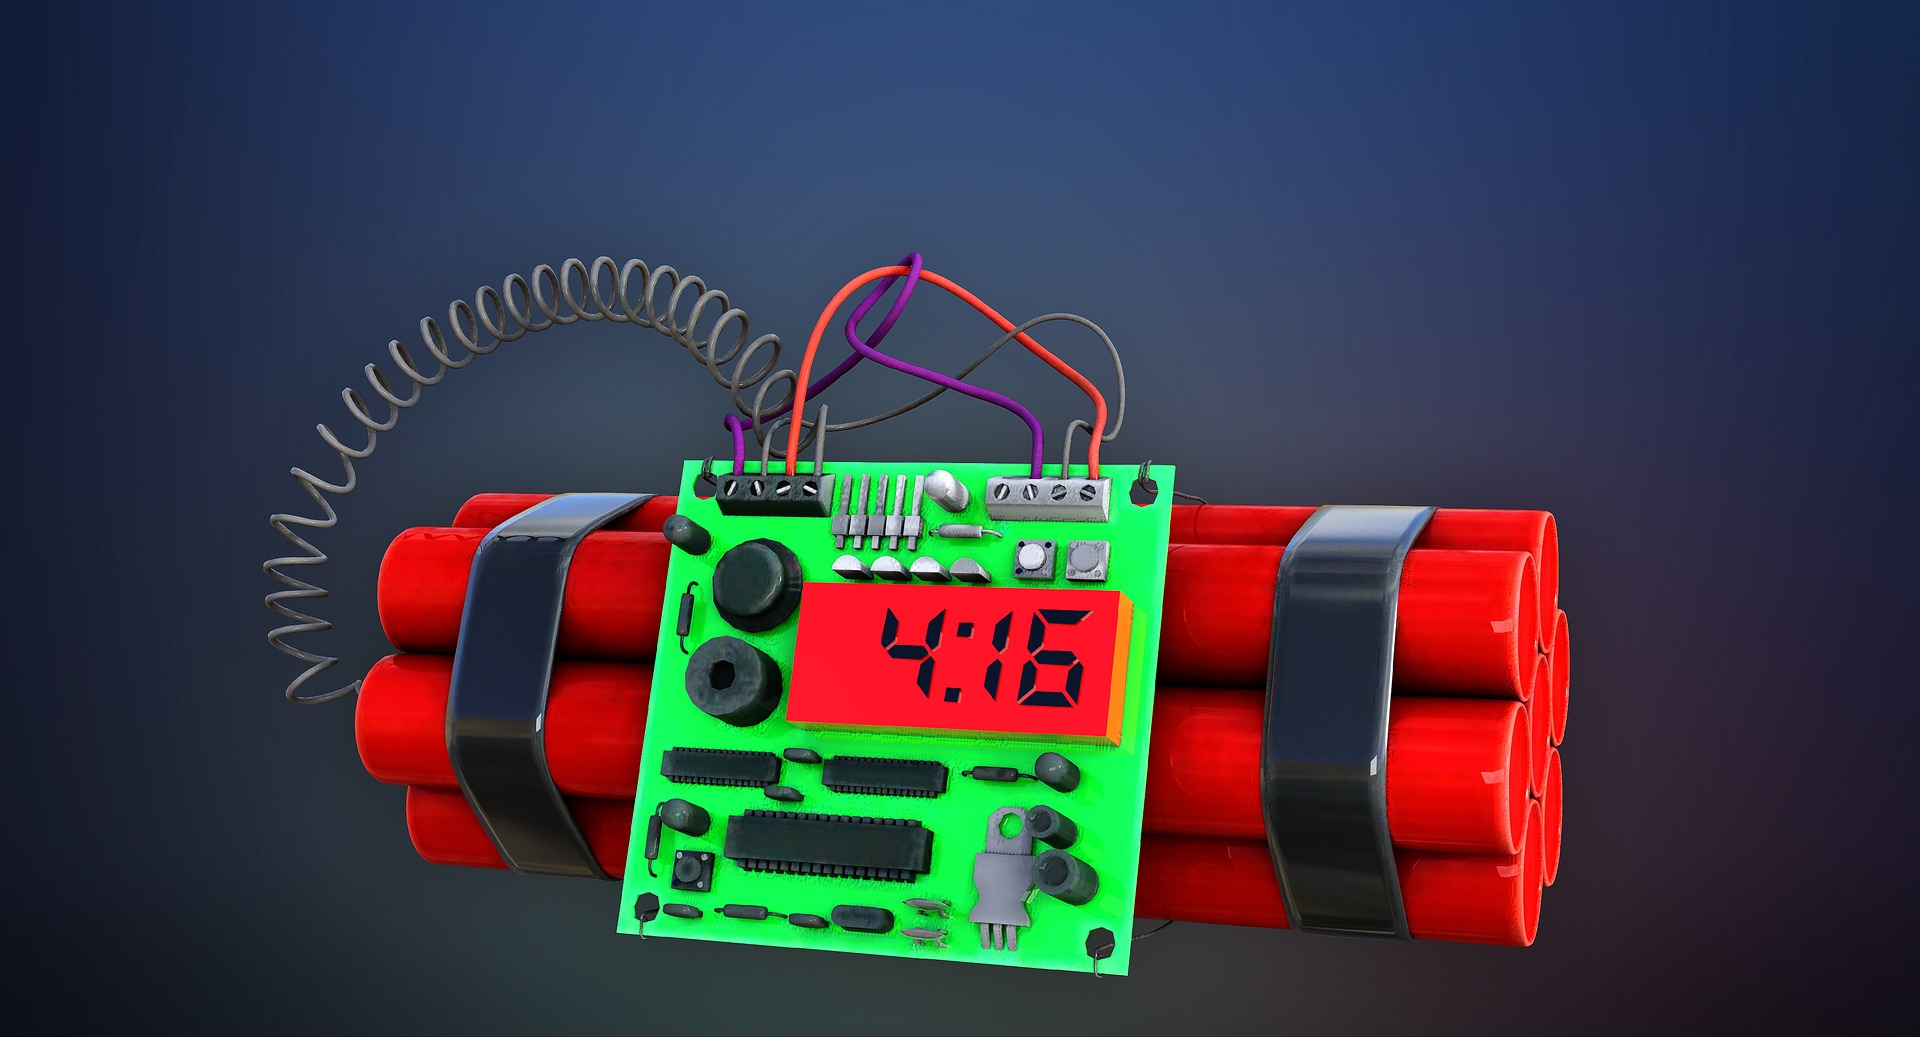
\includegraphics[width=1.0\textwidth]{../img/dynamite}  
\end{SlideExtra}

\begin{SlideExtra}{Undantag orsakar ingen krasch om inkapslad i en Try}
\hspace{0.3\textwidth}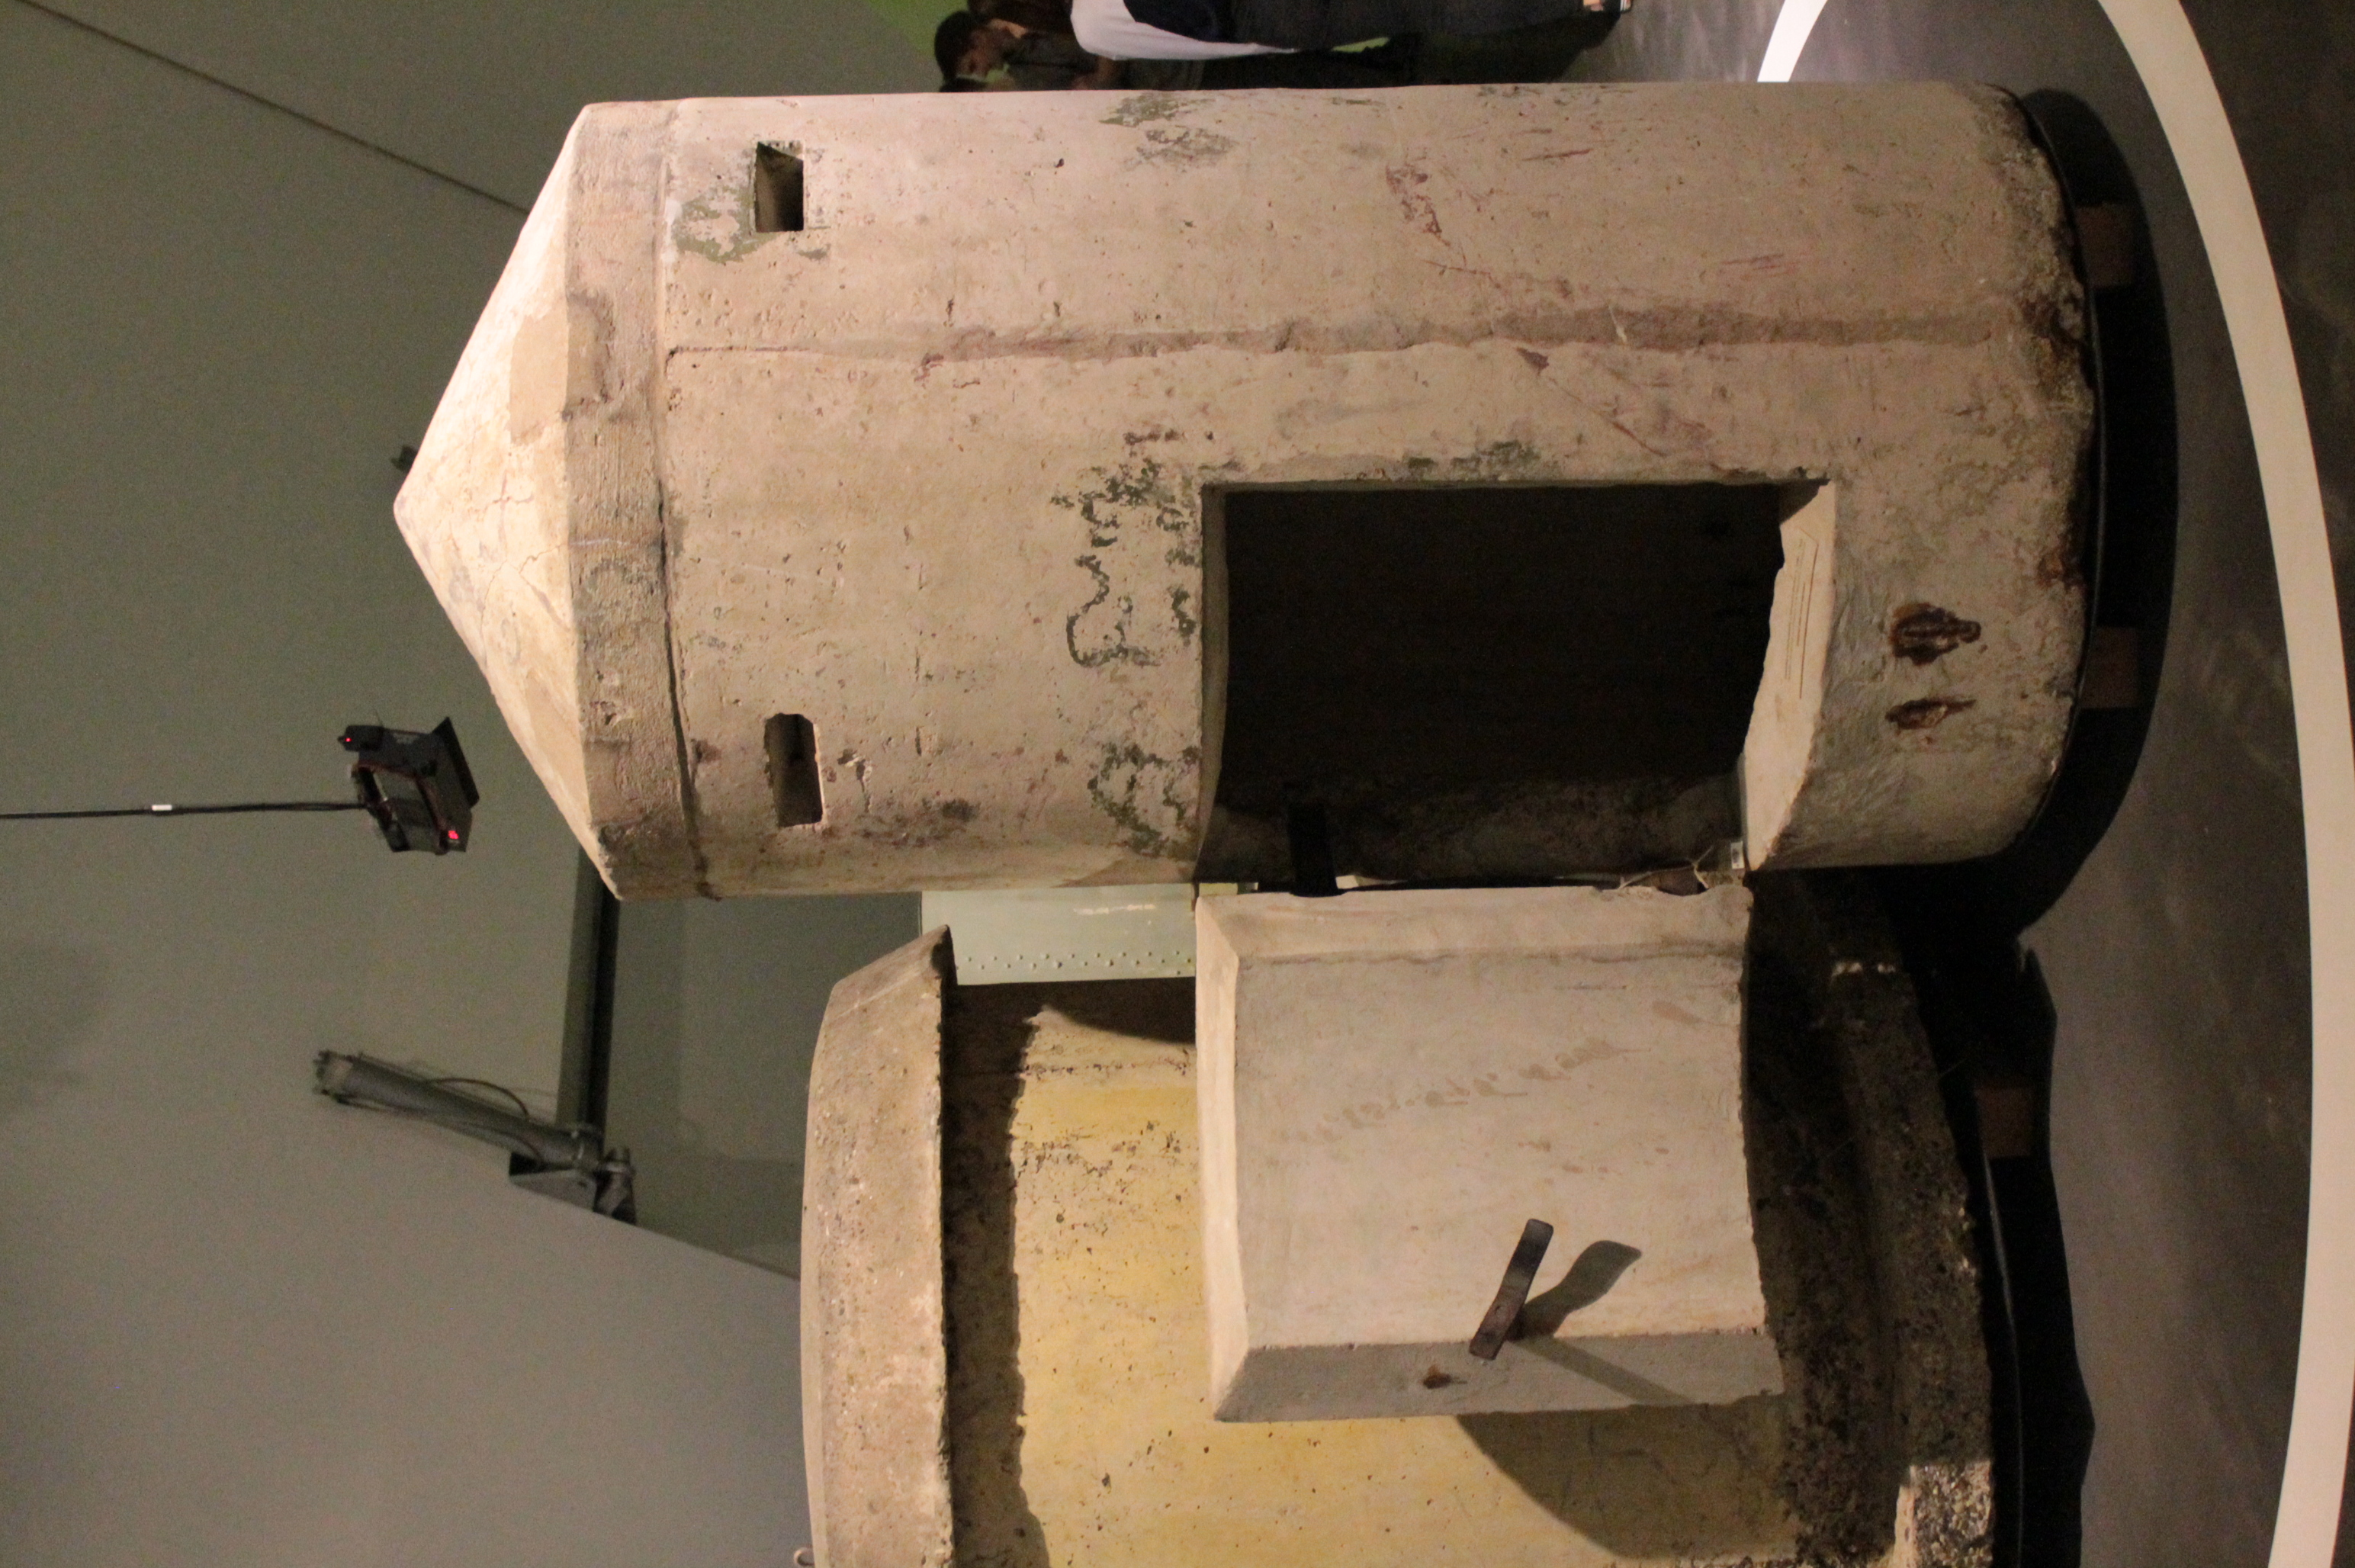
\includegraphics[width=0.6\textwidth,angle=-90,origin=c]{../img/bomb-shelter}  
\end{SlideExtra}
\fi

\begin{Slide}{Vad är ett undantag \Eng{exception}?}
Undantag representerar ett fel eller ett onormalt tillstånd som upptäcks under exekvering och som  behöver hanteras på särskilt sätt vid sidan av det normala exekveringsflödet.

\vspace{1em}\href{https://sv.wikipedia.org/wiki/Undantagshantering}{sv.wikipedia.org/wiki/Undantagshantering}


\vspace{1em} Exempel på undantag:

\pause

\begin{itemize} \SlideFontSmall
\item Indexering utanför vektorns indexgränser.

\item Läsning bortom filens slut.

\item Försök att öppna en fil som inte finns.

\item Minnet är slut.

\item Heltalsdivision med noll ger \code{java.lang.ArithmeticException}.

\item \code{"hej".toInt} ger \code{java.lang.NumberFormatException}

\end{itemize}

\end{Slide}


\begin{Slide}{Orsaka undantag indirekt med \texttt{require} och \texttt{assert}}

\begin{itemize}\SlideFontSmall
  \item Med funktionen \code{require(p)} skapas ett \\\code{IllegalArgumentException("requirement failed")} \\ om \code{p} är \code{false}
  \item \code{require} används om man vill begränsa vilka argument som är giltiga
  \item Med funktionen \code{assert(p)} skapas ett \code{AssertionError("assertion failed")} \\ om \code{p} är \code{false} 
  \item \code{assert} används om man vill förhindra ogiltiga tillstånd
\end{itemize}
{
  \ifkompendium\else
  \vfill\SlideFontTiny
  \fi
  Se implementationen av \code{require} här:\\
\url{https://github.com/scala/scala/blob/v2.13.6/src/library/scala/Predef.scala#L315}
}
\end{Slide}

\begin{Slide}{Kasta dina egna undantag med \texttt{throw}}\SlideFontSmall
Man kan själv generera ett undantag med \code{throw}, vilket kallas att \Emph{kasta} ett undantag som (om det inte \Emph{fångas}), gör att exekveringen \Alert{avbryts}.


\begin{REPL}
scala> def pang = throw Exception("PANG!")
pang: Nothing

scala> pang
java.lang.Exception: PANG!

\end{REPL}
\pause
Olika sätt att hantera undantag och förhindra att exekveringen avbryts:
\begin{itemize}
\item \code{try catch}-uttryck omvandlar undantag till ngt lämpligt värde.
%\item Java: Man kan använda en \code{try ... catch}-sats och \Alert{göra något} i händelse av undantag.

\item \texttt{scala.util.Try} \Emph{kapslar in} kod som kan ge undantag.  %(Finns ej i Java; att föredra i Scala.)
\end{itemize}
\end{Slide}


\Subsection{Hantera undantag med \texttt{Try}}

\begin{Slide}{En gemensam bastyp för något som kan misslyckas}\SlideFontSmall
\begin{Code}
import scala.util.{Try, Success, Failure}
\end{Code}
\ifkompendium\footnotesize\fi
\vspace{-0.5em}\begin{center}
\newcommand{\TextBox}[1]{\raisebox{0pt}[1em][0.5em]{#1}}
\tikzstyle{umlclass}=[rectangle, draw=black,  thick, anchor=north, text width=3.0cm, rectangle split, rectangle split parts = 3]
\begin{tikzpicture}[inner sep=0.5em]
\node [umlclass, rectangle split parts = 2, xshift=0cm, text width=3.8cm] (BaseType)  {
            \textit{\textbf{\centerline{\TextBox{\code{Try[T]}}}}}
            \nodepart[]{second}
            \TextBox{\code{def get: T}}\newline
            \TextBox{\code{def isFailure: Boolean}}\newline
            \TextBox{\code{def isSuccess: Boolean}}
        };

\node [umlclass, rectangle split parts = 2, text width=2.2cm]  at (-2.5cm,-3.7cm) (SubType1) {
            \textbf{\centerline{\TextBox{\code{Success[T]}}}}
            \nodepart[]{second} \TextBox{\code{val value: T}}
        };

\node [umlclass, rectangle split parts = 2, text width=4.2cm] at (2.5cm,-3.7cm) (SubType2)  {
            \textbf{\centerline{\TextBox{\code{Failure[T]}}}}
            \nodepart[]{second} \TextBox{\code{val exception: Throwable}}
        };
\draw[umlarrow] (SubType1.north) -- ++(0,0.5) -| (BaseType.south);
\draw[umlarrow] (SubType2.north) -- ++(0,0.5) -| (BaseType.south);
\end{tikzpicture}
\end{center}
\end{Slide}

\begin{Slide}{Hantera undantag med \texttt{Try}}
\vspace{-0.5em}\begin{REPLsmall}
scala> def pang = throw new Exception("PANG!")

scala> def kanskePang = if math.random() < 0.5 then 42 else pang

scala> import scala.util.{Try, Success, Failure}

scala> def försök = Try { kanskePang }

scala> val xs = Vector.fill(15){försök}

scala> val trettonde = xs(12) match
         case Success(value) => value
         case Failure(e) => println(e); -1

scala> (xs(12).isSuccess, xs(12).isFailure) 

scala> xs(12).getOrElse(0)

scala> xs(12).toOption

scala> försök.foreach(println)

scala> försök.map(_ + 1)

scala> for Success(x) <- xs yield x
\end{REPLsmall}
\end{Slide}

\Subsection{Hantera undantag med \texttt{try}-\texttt{catch}}


\begin{Slide}{\texttt{try}-\texttt{catch}-uttryck}\SlideFontSmall
Man kan fånga undantag med ett \code{try ... catch}-uttryck:
\begin{Code}
def carola = 
  try 
    if math.random() > 0.5 then throw Exception("stormvind")
    42
  catch 
    case e: Exception =>
      println("Fångad av en " + e.getMessage)
      -1

\end{Code}
\pause
\begin{REPL}
scala> Vector.fill(5)(carola)
Fångad av en stormvind
Fångad av en stormvind
Fångad av en stormvind
val res0: Vector[Int] = Vector(-1, 42, 42, -1, -1)
\end{REPL}
%Gör uppg. 9-11 i övn. \code{patterns} som visar hur man fångar undantag i Scala och Java. 
%Mer om undantag i fortsättningskursen.
\end{Slide}

%!TEX encoding = UTF-8 Unicode
%!TEX root = ../lect-w06.tex

%%%

\Subsection{Fördjupning: Implementera \texttt{equals}}

\ifkompendium
\noindent När du jämför värden med \code{==} anropas metoden \code{equals} som finns för alla typer. Du kan i dina egna klasser överskugga \code{equals} med en din egna definition av vad likhet ska innebära. Då är det lämpligt att använda matchning. Det är dock ett ganska omfattande arbete att implementera en korrekt likhetsjämförelse som fungerar under alla omständigheter. Ett recept för en fullständig implementation av \code{equals} ges i fördjupningen nedan. 
\fi

\begin{Slide}{Fördjupning: Implementera \texttt{equals} med \texttt{match}}
Det visar sig att \Emph{innehållslikhet} är \Alert{förvånansvärt komplicerat} att implementera, speciellt  i samband med arv.
\begin{itemize}\SlideFontSmall
\item Det enklare fallet: Gör fördjupningsuppgift \textit{''Metoden \code{equals}''} och implementera \code{equals} för innehållslikhet utan arv. \\ En bra träning på att använda \code{match}!

\item Svårare: Gör fördjupningsuppgifterna  \textit{''Överskugga \code{equals}''} och \textit{''Överskugga equals vid arv''} om du vill se hur en \Emph{komplett} \code{equals} ska se ut som fungerar \Alert{i alla lägen}.

\end{itemize}

\noindent Det krävs i denna kurs inte att du själv ska kunna implementera en generellt fungerande \code{equals}. Men du ska förstå skillnaden mellan referenslikhet och innehållslikhet. Mer om \code{equals} i fortsättningkursen, men en liten inblick i problemet nu...
\end{Slide}

\ifkompendium
\noindent Om en klass markeras \code{final} kan den ej ha några subklasser. Kompilatorn kontrollerar att detta gäller alla finala klasser och ger kompileringsfel om du försöker göra \code{extends} på en final klass. Om en klass garanterat inte har några subklasser kan implementationen av \code{equals} göra enklare.
\fi 

\begin{Slide}{Fördjupning: \texttt{equals} som fungerar för finala klasser}
Recept för implementation av \code{equals} som fungerar för typer som \Alert{inte} har några subtyper:
\begin{Code}
final class Gurka(val vikt: Int, val ärÄtbar: Boolean):
  override def equals(other: Any): Boolean = other match
    case that: Gurka => vikt == that.vikt && ärÄtbar == that.ärÄtbar
    case _ => false

  override def hashCode: Int = (vikt, ärÄtbar).## // ger bra hashcode
\end{Code}
\begin{itemize}\SlideFontSmall
\item
Du \Alert{måste} alltid överskugga \code{hashCode} också om du överskuggar \code{equals} annars funkar inte gurksamlingar (lång story ...)
\item
Notera typen \code{Any} -- detta följer hur man valde att göra i Java (tyvärr?).
\pause
\item
Ett \Alert{typsäkrare} innehållslikhetstest som \Emph{garanterat} bara jämför en gurka med en gurka och inget annat:
\begin{Code}
def ===(other: Gurka): Boolean =
  vikt == other.vikt && ärÄtbar == other.ärÄtbar
\end{Code}
\end{itemize}
\end{Slide}


\begin{Slide}{Fördjupning: Recept i 8 steg för arvssäker \code{equals}}\SlideFontTiny
%fungerar även för klasser som inte är \code{final}:
\SlideOnly{\setlength{\leftmargini}{0pt}}
\begin{enumerate}\SlideFontTiny
\item Inför denna metod: \code{ def canEqual(other: Any): Boolean}\\Observera att typen på parametern ska vara \code{Any}. Om subklass behövs \code{override}.

\item Metoden \code{canEqual} ska ge \code{true} om \code{other} är av samma typ som \code{this}, t.ex.: \\\code{override def canEqual(other: Any): Boolean = other.isInstanceOf[Gurka]}

\item Inför metoden \code{equals} och var noga med att parametern har typen \code{Any}: \\ \code{override def equals(other: Any): Boolean}

\item Implementera metoden \code{equals} med ett match-uttryck som börjar så här: \\
\code|other match { ... } |

\item Match-uttrycket ska ha två grenar. Den första grenen ska ha ett typat mönster för den klass som ska jämföras, t.ex.: \\ \code{  case that: Gurka =>}

\item Om du implementerar \code{equals} i den klass som inför \code{canEqual}, börja med: \\ \code{(that canEqual this) &&} \\
och skapa därefter en fortsättning som baseras på innehållet i klassen, t.ex.: \\ \code{this.vikt == that.vikt && this.längd == that.längd} \\
Om du överskuggar equals vill du nog börja med
 \code{super.equals(that) && }

\item Den andra grenen i matchningen ska vara:
\code{case _ => false}

\item Överskugga \code{hashCode}, t.ex. med tupel av attributvärden och metoden \code{##}: \\
\code{override def hashCode: Int  = (vikt, längd).## }

\end{enumerate}
\url{http://www.artima.com/pins1ed/object-equality.html}

\end{Slide}


\begin{Slide}{Fördjupning: Säkrare likhetstest i Scala 3}
\SlideFontSmall
\begin{itemize}
\item \Alert{Problem}: \code{equals} tar värden av vilken typ som helst.
\item Detta kallas \Alert{universell likhet}.
\item[]
\begin{REPLsmall}
scala> case class Hund(namn: String)
scala> case class Katt(namn: String)
scala> Hund("bob") == Katt("bob") // knasig jämförelse; kan aldrig bli sant
val res0: Boolean = false         // men kompilatorn låter dig göra likhetstestet
\end{REPLsmall}  
\item I Scala 3 kan du få typsäker likhetstest med~~\code{derives CanEqual}
\item Detta kalla \Emph{multiversell likhet}.
\item[]
\begin{REPLsmall}
scala> case class Hund(namn: String) derives CanEqual
scala> Hund("bob") == Katt("bob")   // tack kompilatorn för fel:
-- Error:
1 |Hund("bob") == Katt("bob")
  |^^^^^^^^^^^^^^^^^^^^^^^^^^
  |Values of types Hund and Katt cannot be compared with == or !=
\end{REPLsmall}  
\item Du \Emph{slipper} skriva \code{derives CanEqual} om du gör: \\ \code{import scala.language.strictEquality}
\item Läs mer här: \url{https://docs.scala-lang.org/scala3/reference/contextual/multiversal-equality.html}

\end{itemize}

\end{Slide}

%!TEX encoding = UTF-8 Unicode
%!TEX root = ../lect-w06.tex

%%%

\ifkompendium\else
\Subsection{Veckans uppgifter}

\begin{SlideExtra}{Veckans övning: \texttt{patterns}}
  Mål: Träna på matchning och undantag
\begin{itemize}
\item Uppg. 1--8: Matchning, \code{Option}
\item Uppg. 9--11: Undantag, \code{Try}
\item Uppg. 12: Laborationsförberedelse \code{Cell} och \code{Table}
\item Uppg. 13: Matchning eller dynamisk bindning?
\item Uppg. 14: avgöra likhet med matchning, \code{equals} utan arv
\item Uppg. 15--22: diverse fördjupningsuppgifter om matchning, undantag, hash-koder, likhet vid arvshierarki
\end{itemize}
\end{SlideExtra}


\begin{SlideExtra}{Veckans labb: \texttt{tabular}}\SlideFontTiny
%  \setlength{\leftmargini}{0pt}
\hspace{-2em}\begin{minipage}{0.7\textwidth}
\vspace{0.25em}
\Emph{Förberedelse:}
\begin{itemize}
\item Gör övning \code{patterns}, speciellt uppg. 12
\item Studera givna koden: {\SlideFontTiny \href{https://github.com/lunduniversity/introprog/tree/master/workspace/w13_tabular}{workspace/w10\_tabular}}
\item Fyll i denna enkät:
\\{\SlideFontTiny \url{https://goo.gl/forms/hC6JK2UQXVpbGECc2}}
\item Se svar här (snapshot uppdateras då och då): \url{http://cs.lth.se/pgk/favorit}
\end{itemize}

\Emph{Grunduppgift:}
\begin{itemize}
\item Terminalapp för hantering av kolumndata i textfiler.
\item Matchning används vid kommandotolkning.
\item \code{Option} används för inkapsling av ev. saknade värden
\item \code{Try} används för inkapsling av ev. undantag
\end{itemize}
\Emph{Extrauppgifter:} (Minst en)
\begin{itemize}
\item dialoger: \code{load}, \code{save}, kommando: \code{pie}, \code{bar}
\end{itemize}
\end{minipage}
\hfill\begin{minipage}{0.3\textwidth}
\centering
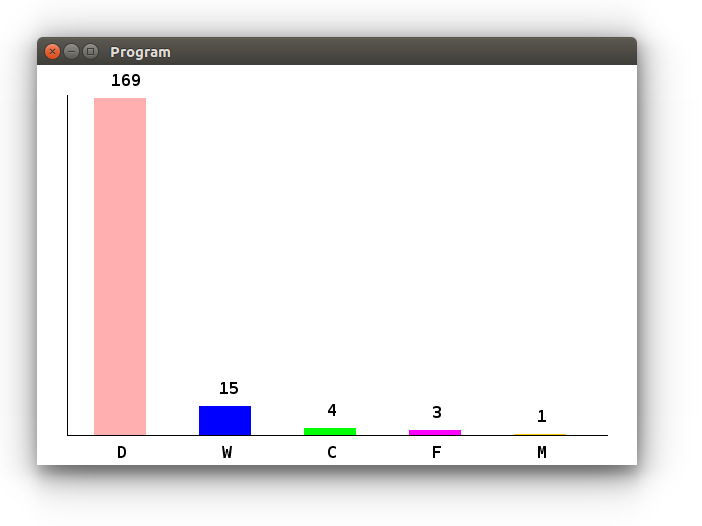
\includegraphics[width=0.95\textwidth]{../img/survey/bar}

\vspace{2em}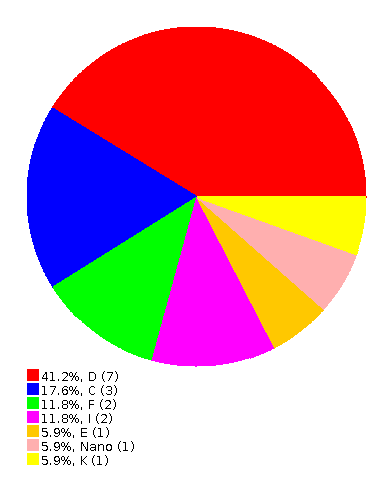
\includegraphics[width=0.7\textwidth]{../img/survey/pie}
\end{minipage}
\end{SlideExtra}

\begin{SlideExtra}{Extraundervisning del 3}
\begin{itemize}
\item  \Alert{Extraundervisning} i \Emph{E:1406} onsdag 21/11 kl 15:15-17:00
\item Hitta dit: \url{http://fileadmin.cs.lth.se/ehus/E1406.pdf}
\item Det finns gott om platser i den salen >70 platser så alla är välkomna
\item Fokus: grundläggande, långsam behandling på begäran, grumliga begrepp etc.
\end{itemize}
\end{SlideExtra}
\fi



\end{document}
 